% =====================================================================
% Main LaTeX document for SOICT submission
% Title: SE2RoadNet: A Geometry- and Physics-Grounded Transformer
%        for Robust Test Prioritization in Self-Driving Cars
% =====================================================================

% For SOICT / ACM ICPS format, use:
% \documentclass[sigconf,screen]{acmart}

% Fallback / Local compilation using IEEEtran:
\documentclass[conference]{IEEEtran}
\IEEEoverridecommandlockouts

\usepackage{cite}
\usepackage{amsmath,amssymb,amsfonts,amsthm}
\usepackage{graphicx}
\graphicspath{{figures/}{../figures/}{../../presentation/figures/}}
\usepackage{textcomp}
\usepackage{xcolor}
\usepackage{booktabs}
\usepackage{hyperref}
\usepackage{tikz}
\usetikzlibrary{positioning,fit,backgrounds,arrows.meta}
\usepackage{pifont}
\usepackage{multirow}
\usepackage{array}

\newcommand{\cmark}{\ding{51}}
\newcommand{\xmark}{\ding{55}}
\newcommand{\softred}[1]{\textcolor{red!70!black}{#1}}
\newcommand{\softgreen}[1]{\textcolor{green!60!black}{#1}}

\begin{document}

\title{SE2RoadNet: A Geometry- and Physics-Grounded Transformer for Robust Test Prioritization in Self-Driving Cars}

\author{
\IEEEauthorblockN{
Chi-Nguyen Tran$^*$,
Dao Sy Duy Minh$^*$,
Huynh Trung Kiet$^*$,
Phu-Hoa Pham,
Nguyen Lam Phu Quy
}
\IEEEauthorblockA{\textit{Faculty of Information Technology, University of Science (HCMUS), Vietnam}}
\IEEEauthorblockA{\textit{Vietnam National University -- Ho Chi Minh City (VNU-HCM), Vietnam}}
\IEEEauthorblockA{\{23122044, 23122041, 23122039, 23122030, 23122048\}@student.hcmus.edu.vn}
\IEEEauthorblockA{$^*$Equal contribution}
}

\maketitle

\begin{abstract}
Simulation-based testing is indispensable for evaluating autonomous driving systems, yet executing long trajectories in high-fidelity simulators is computationally prohibitive. Test case prioritization seeks to maximize early fault detection (APFD), but existing deep learning approaches suffer from three fundamental vulnerabilities: they are sensitive to arbitrary coordinate rotations, brittle under simulator point-sampling shifts, and prone to unphysical failure predictions.
In this work, we propose \textbf{SE2RoadNet}, an advanced geometry- and physics-grounded Transformer for self-driving car test prioritization that directly addresses these vulnerabilities. 
SE2RoadNet preserves the full sequential road geometry through seven intrinsic, coordinate-free differential geometric features, guaranteeing exact $\mathrm{SE}(2)$ rigid-motion invariance via a relative-arclength attention bias parameterized by Random Fourier Features. 
Furthermore, we incorporate a physics-informed neural network (PINN) regularization term based on vehicle dynamics limits, ensuring that predicted risk is monotone with respect to peak centripetal acceleration.
Extensive experiments across eight public benchmarks and SensoDat (32,580 tests) demonstrate that SE2RoadNet achieves exact rotation invariance ($\Delta\mathrm{APFD} = 0.0000$), discretization invariance ($\Delta\mathrm{APFD} \le 0.0012$), and a $5.6\times$ reduction in physical curvature violations, while consistently outperforming heuristic, machine learning, and deep sequence baselines with an APFD of $0.805$--$0.807$ and a state-of-the-art AUC of $0.935$.
\end{abstract}

\begin{IEEEkeywords}
Test prioritization, self-driving cars, SE(2)-equivariance, physics-informed neural networks, Transformer, autonomous driving simulation.
\end{IEEEkeywords}

% ---------------------------------------------------------------------
% Content Sections
% ---------------------------------------------------------------------

\section{Introduction}
\label{sec:intro}

Simulation-based testing is vital for verifying safety-critical Autonomous Cyber-Physical Systems (ACPS), ranging from Autonomous Driving Systems (ADS) to Unmanned Aerial Vehicles (UAVs)~\cite{sdcscissor,sensodat}.
High-fidelity physics simulators (e.g., BeamNG.tech and Gazebo/PX4) allow engineers to evaluate control policies across hazardous corner cases without risking physical damage.
However, simulating multi-agent interactions, sensor telemetry, and nonlinear friction forces is computationally prohibitive.
A realistic verification suite containing thousands of test scenarios requires hundreds of machine-hours to execute.
To mitigate this bottleneck, \emph{test case prioritization} (TCP)~\cite{apfd,yooharman} reorders test suites so that failure-revealing scenarios are executed as early as possible.
Prioritization performance is standardly evaluated via the Average Percentage of Faults Detected (APFD)~\cite{apfd}:
\begin{equation}
\mathrm{APFD}(\pi) = 1 - \frac{\sum_{i=1}^{m} TF_i}{n \cdot m} + \frac{1}{2n},
\label{eq:apfd}
\end{equation}
where $n$ is the total number of test cases, $m$ is the count of failing test cases, and $TF_i$ is the rank position of the first test exposing fault $i$.
An ideal prioritization yields an APFD approaching $1.0$, whereas random execution yields $\approx 0.50$.

Existing approaches to autonomous system test prioritization broadly fall into three categories:
(i)~\emph{Heuristic and search-based diversification} (e.g., SDC-Prioritizer~\cite{sdcprio} and Surrealist~\cite{roadfury}), which employ genetic algorithms to maximize behavioral or static diversity;
(ii)~\emph{Feature-based machine learning} (e.g., SDC-Scissor~\cite{sdcscissor,saner}), which extracts hand-crafted tabular descriptors (such as turn counts, bounding box areas, and mean curvatures); and
(iii)~\emph{Deep sequence models} (e.g., ITS4SDC~\cite{its4sdc} and RoadFury~\cite{roadfury}), which process waypoint sequences using LSTMs or Transformers.
While deep sequence architectures achieve strong APFD ($\approx 0.807$), a critical examination reveals four foundational limitations:
\begin{enumerate}
    \item \textbf{Coordinate Frame Fragility}: Existing neural prioritizers rely on extrinsic coordinate features (Cartesian coordinates $(x, y, z)$ or yaw angles). Consequently, rotating a scenario's global coordinate frame induces severe rank drift ($\Delta\mathrm{APFD} > 0.05$), even though the underlying physical trajectory is identical.
    \item \textbf{Discretization Sensitivity}: Simulators frequently alter trajectory waypoint sampling frequencies. Fixed-rate neural networks suffer performance degradation when evaluated on resampled curves.
    \item \textbf{Unphysical Failure Predictions}: Standard statistical loss functions treat risk prediction as unconstrained pattern matching, frequently producing non-monotonic predictions where sharper curves or extreme aerodynamic gusts are paradoxically predicted as less hazardous.
    \item \textbf{Lack of Statistical Guarantees}: Existing prioritizers provide heuristic rankings with zero finite-sample safety assurances, leaving test engineers without rigorous stopping criteria.
\end{enumerate}

To resolve these limitations, we propose \textbf{CliffordTrajNet}, a unified geometric deep learning and continuous state-space framework for test prioritization across autonomous vehicles and UAVs.
First, CliffordTrajNet formulates spatial trajectories in Clifford Geometric Algebra $C\ell(p, q)$ ($C\ell(2,0)$ for 2D road driving and $C\ell(3,0)$ for 3D aerial flight).
By operating on grade-preserving multivectors and rotor sandwich operations ($v' = R v R^\dagger$), CliffordTrajNet guarantees exact planar $SE(2)$ invariance and substantially reduces 3D spatial sensitivity without gimbal lock.
Second, we incorporate a continuous-time Selective State Space Model (\textbf{TrajMamba}) driven by arclength ODE integration ($\Delta t = \Delta s / v$), substantially reducing discretization sensitivity across variable waypoint densities.
Third, we formulate a physics-informed monotonicity regularizer enforcing curvature monotonicity, reducing unphysical predictions by $5.6\times$.
Finally, we integrate \textbf{Monotone Conformal Risk Control} (CRC), providing finite-sample probably approximately correct (PAC) statistical bounds that guarantee test failure miss-rates remain bounded under tight execution budgets.

In summary, this paper presents the following contributions:
\begin{itemize}
    \item \textbf{Invariant Clifford Geometric Foundations}: We formulate test prioritization in Clifford Geometric Algebra, guaranteeing exact $SE(2)$ invariance on ground roads ($\Delta\mathrm{APFD} = 0.0000$) and high spatial robustness on 3D UAV paths ($\Delta\mathrm{APFD} \le 0.0119$).
    \item \textbf{Continuous State-Space Dynamics (TrajMamba)}: We achieve strong robustness against waypoint discretization sensitivity ($\Delta\mathrm{APFD} \le 0.0012$) via continuous arclength ODE integration over variable-resolution trajectories.
    \item \textbf{PAC Safety Bounds}: We establish rigorous stopping criteria, showing that allocating just $17.05\%$ budget catches $\ge 98.72\%$ of critical simulation failures on evaluated benchmarks.
    \item \textbf{Extensive Cross-Domain Evaluation}: Across 32,580 SensoDat simulation tests, nine external SDC benchmarks, and the official SBFT 2026 UAV benchmark, CliffordTrajNet achieves the highest AUC among evaluated methods ($0.9399$) while matching the strongest APFD performance ($0.8063$ vs. $0.8066$ for RoadFury), outperforming heuristic, tabular, and deep learning baselines.
\end{itemize}

\section{Related Work}
\label{sec:related}

Prioritizing simulation-based tests for self-driving cars (SDCs) has been investigated from three main paradigms: (i)~\emph{search-based and diversity} methods that reorder test suites to maximize behavioral or static distance, (ii)~\emph{feature-based machine learning} that scores roads via hand-engineered tabular statistics, and (iii)~\emph{deep sequence learning} that processes raw geometry end-to-end. 
In this section, we review each paradigm, analyze the theoretical foundations of group equivariance and physical regularization, and position SE2RoadNet within the literature.

\subsection{Search-Based and Diversity-Driven Prioritization}

SDC-Prioritizer~\cite{sdcprio} formulates test case prioritization as a black-box combinatorial optimization problem.
A chromosome $\pi = \langle t_1, \dots, t_n \rangle$ represents a candidate execution order, evolved via genetic algorithms to ensure that diverse and computationally inexpensive tests are scheduled first.
The single-objective variant maximizes a cost-discounted diversity metric:
\begin{equation}
f(\pi) = \sum_{i=2}^{n} \frac{\mathrm{dist}(t_i, t_{i-1})}{\mathrm{cost}(t_i) \cdot i},
\end{equation}
where $\mathrm{dist}(t_i, t_{i-1})$ denotes the Euclidean distance between $z$-normalized static road feature vectors, and the multiplier $i$ prioritizes early fault detection.
The multi-objective variant (MO-SDC-Prioritizer) uses NSGA-II to optimize diversity and execution cost simultaneously.
While search-based prioritization requires no historical failure labels and operates with minimal runtime overhead ($<0.5\%$), diversity serves only as an indirect surrogate for fault-revealing capability.
Crucially, global Euclidean distance over hand-crafted features provides neither rotational invariance nor sampling-rate consistency.

\subsection{Feature-Based Machine Learning}

SDC-Scissor~\cite{sdcscissor,saner} predicts unsafe scenarios prior to simulation by extracting static descriptors---such as turn counts, min/max/mean turn angles, pivot radii, total length, and Shapely polygon bounding areas---and feeding them into tabular classifiers (Logistic Regression, Random Forest, Gradient Boosting).
Although SDC-Scissor reports cost-effectiveness gains of up to $4.0\times$ by filtering out benign scenarios, it suffers from two structural weaknesses:
First, counting features (e.g., number of left/right turns) depend on an arbitrary spline segmentation threshold; resampling the road alters these descriptors.
Second, aggregating roads into scalar summaries erases the localized spatial transitions where sudden steering adjustments induce vehicle spinouts.

\subsection{Deep Sequence Models}

To capture fine-grained geometry, recent research has turned to deep neural networks.
ITS4SDC~\cite{its4sdc} models roads as sequences of per-segment relative turn angles and lengths $(\Delta\theta_k, \ell_k)$ using a bi-directional LSTM (220 units), reaching an $F_1$-score of $0.89$ in the ICST 2025 competition.
Setting the initial heading to zero partially mitigates global orientation bias, but remains a heuristic rather than an architectural invariance guarantee.
Furthermore, the LSTM's rigid sequence dimension ($N=197$) ties predictions to a specific discretization rate.

Our earlier baseline, RoadFury~\cite{roadfury}, introduced a 4-layer Pre-LN Transformer Encoder~\cite{transformer,preln} with Stochastic Weight Averaging (SWA)~\cite{swa} trained on a 10-channel geometric matrix.
While RoadFury won the ICST 2026 competition with an APFD of $0.804 \pm 0.012$, its feature set retained frame-dependent components ($\sin\theta, \cos\theta, \theta$) and absolute sinusoidal positional embeddings, making it vulnerable to coordinate rotation and scale shifts.

\subsection{Theoretical Foundations: Invariance and Physics Grounding}

\textbf{Group Equivariance}: 
A mapping $\Phi: \mathcal{X} \to \mathcal{Y}$ is equivariant to a transformation group $G$ if $\Phi(T_g x) = T'_g \Phi(x)$ for all $g \in G$~\cite{gcnn}.
When the target space is invariant ($T'_g = \mathrm{Id}$), the output satisfies $\Phi(T_g x) = \Phi(x)$.
Standard Group Equivariant CNNs~\cite{gcnn} operate over discrete planar rotations ($p4$ or $p4m$ symmetries on 2D pixel grids) and cannot provide continuous $\mathrm{SE}(2)$ rigid-motion invariance for continuous 1D spatial curves.
In contrast, by the fundamental theorem of planar curves~\cite{frenet}, a regular curve is uniquely determined up to a rigid motion by its signed curvature $\kappa(s)$ parameterized by arclength $s$.
By designing an attention mechanism conditioned solely on intrinsic differential curvature and relative arclength intervals $\Delta s = |s_i - s_j|$ via Random Fourier Features (RFF)~\cite{rff}, SE2RoadNet achieves continuous, exact $\mathrm{SE}(2)$ invariance.

\textbf{Physics-Informed Regularization}:
In autonomous vehicle dynamics, lateral wheel slip occurs when centripetal acceleration exceeds available tire-road friction: $a_c = v^2 \kappa(s) > \mu g$.
Physics-Informed Neural Networks (PINN)~\cite{pinn} integrate physical conservation laws into neural loss functions.
In this work, we embed the physical friction limit directly into the prioritization objective, penalizing predictions where high-risk scores are assigned to low-curvature trajectories.

\subsection{Positioning}

Table~\ref{tab:positioning} contrasts SE2RoadNet against representative prior approaches.
While empirical APFD has largely plateaued around $0.80$, SE2RoadNet is the first framework to provide both architectural $\mathrm{SE}(2)$ invariance and physics-grounded curvature monotonicity.

\begin{table}[t]
\caption{Comparison of SDC Test Prioritization Approaches.}
\label{tab:positioning}
\centering{\small
\setlength{\tabcolsep}{4pt}
\begin{tabular}{llccc}
\toprule
\textbf{Method} & \textbf{Paradigm} & \textbf{APFD} & \textbf{$\mathrm{SE}(2)$-Inv.} & \textbf{Physics Loss} \\
\midrule
Random & Baseline & $\approx 0.50$ & \xmark & \xmark \\
SO-SDC-Prioritizer~\cite{sdcprio} & Search & $\approx 0.77$ & \xmark & \xmark \\
Greedy Diversity~\cite{sdcprio} & Search & $\approx 0.80$ & \xmark & \xmark \\
SDC-Scissor~\cite{sdcscissor} & Tabular ML & $\approx 0.75$ & \xmark & \xmark \\
ITS4SDC~\cite{its4sdc} & Deep (LSTM) & $\approx 0.78$ & \xmark & \xmark \\
RoadFury~\cite{roadfury} & Deep (Transf.) & $\approx 0.81$ & \xmark & \xmark \\
\textbf{SE2RoadNet (Ours)} & \textbf{Deep (Transf.)} & \textbf{$\approx 0.81$} & \textbf{\cmark} & \textbf{\cmark} \\
\bottomrule
\end{tabular}}
\end{table}

\section{Methodology}
\label{sec:method}

In this section, we present the mathematical formulation and structural design of \textbf{SE2RoadNet}.
We first define the planar curve representation and formalize the requirement for $\mathrm{SE}(2)$ rigid-motion invariance.
We then detail the 7-channel coordinate-free feature set, the relative-arclength attention bias mechanism, and the physics-informed regularizer.

\subsection{Problem Formulation and Invariance Guarantee}

Let a test scenario road trajectory be represented as a continuous planar curve $\mathbf{r}(s) = (x(s), y(s))^\top \in \mathbb{R}^2$, parameterized by its arclength $s \in [0, L]$.
In practice, the road is discretized into a polyline of $L$ control points $\mathcal{P} = \{\mathbf{p}_1, \dots, \mathbf{p}_L\}$, where $\mathbf{p}_i \in \mathbb{R}^2$.
The objective of test prioritization is to learn a scoring function $f: \mathcal{P} \to [0, 1]$ that estimates the probability of simulation failure, inducing a permutation $\pi$ that sorts test cases in descending order of predicted risk.

The physical vehicle dynamics in an autonomous driving simulation (friction, tire-road lateral forces, and lane deviation) are completely independent of the arbitrary world coordinate frame in which the road is embedded.
Formally, let $g = (\mathbf{R}, \mathbf{t}) \in \mathrm{SE}(2)$ denote a rigid planar motion consisting of a rotation matrix $\mathbf{R} \in \mathrm{SO}(2)$ and a translation vector $\mathbf{t} \in \mathbb{R}^2$.
The transformed road points are given by:
\begin{equation}
T_g(\mathbf{p}_i) = \mathbf{R} \mathbf{p}_i + \mathbf{t}.
\end{equation}
A prioritization scoring model $f$ is defined to be \emph{$\mathrm{SE}(2)$-invariant} if and only if:
\begin{equation}
f(T_g(\mathcal{P})) = f(\mathcal{P}) \quad \forall g \in \mathrm{SE}(2).
\label{eq:se2_def}
\end{equation}
When Eq.~\eqref{eq:se2_def} holds, the resulting ranking $\pi$ is identical under all rotations and translations, precluding artificial ranking variance.

\subsection{Intrinsic Coordinate-Free Feature Set}

Prior deep architectures incorporate absolute headings $\theta_i$ or trigonometric components $(\sin\theta_i, \cos\theta_i)$.
Under a planar rotation $\mathbf{R}_\alpha$ by angle $\alpha$, the heading transforms as $\theta'_i = \theta_i + \alpha$, which directly shifts input activations and destroys invariance.

To achieve exact invariance, SE2RoadNet extracts seven differential geometric invariants that depend solely on intrinsic curve geometry (Table~\ref{tab:features}).
By the fundamental theorem of planar curves~\cite{frenet}, any smooth curve is uniquely determined up to an $\mathrm{SE}(2)$ transformation by its signed curvature $\kappa(s)$.
Given three consecutive points $\mathbf{p}_{i-1}, \mathbf{p}_i, \mathbf{p}_{i+1}$, we compute the signed Menger curvature:
\begin{equation}
\kappa_i = \frac{4 A_i}{a_i b_i c_i} \cdot \mathrm{sgn}\left(\det[\mathbf{p}_i - \mathbf{p}_{i-1}, \;\mathbf{p}_{i+1} - \mathbf{p}_i]\right),
\end{equation}
where $a_i, b_i, c_i$ are triangle side lengths and $A_i$ is the triangle area computed via Heron's formula.
The complete feature vector at control point $i$ is $\mathbf{x}_i = [f_0(i), \dots, f_6(i)]^\top \in \mathbb{R}^7$.
Crucially, every channel $f_k(i)$ satisfies $f_k(T_g(\mathbf{p}_i)) = f_k(\mathbf{p}_i)$ for all $g \in \mathrm{SE}(2)$.

\begin{table}[t]
\caption{The 7-Channel Coordinate-Free Feature Set of SE2RoadNet.}
\label{tab:features}
\centering{\small
\setlength{\tabcolsep}{4pt}
\begin{tabular}{clll}
\toprule
\textbf{Ch.} & \textbf{Feature} & \textbf{Mathematical Definition} & \textbf{Physical Meaning} \\
\midrule
$f_0$ & Segment length & $\ell_i = \|\mathbf{p}_{i+1} - \mathbf{p}_i\|_2$ & Local discretization \\
$f_1$ & Turn angle & $|\Delta\theta_i| = \arccos\left(\frac{\mathbf{v}_i \cdot \mathbf{v}_{i+1}}{\|\mathbf{v}_i\|\|\mathbf{v}_{i+1}\|}\right)$ & Bending intensity \\
$f_2$ & Signed curvature & $\kappa_i = 4 A_i / (a_i b_i c_i) \cdot \mathrm{sgn}(\Delta)$ & Lateral acceleration factor \\
$f_3$ & Curvature jerk & $\Delta\kappa_i / \ell_i = (\kappa_{i+1} - \kappa_i) / \ell_i$ & Rate of steering change \\
$f_4$ & Curvature accel. & $\Delta^2\kappa_i / \ell_i^2$ & Steering impulse \\
$f_5$ & Arclength norm. & $s_i / L_{\text{tot}} = \sum_{j=1}^i \ell_j / L_{\text{tot}}$ & Relative trajectory progress \\
$f_6$ & Local curv. std & $\mathrm{std}(\kappa_{i-w:i+w})$ & Curvature volatility ($w=5$) \\
\bottomrule
\end{tabular}}
\end{table}

\subsection{SE2RoadNet Transformer Architecture}

Fig.~\ref{fig:arch_se2} illustrates the complete pipeline of SE2RoadNet.

\begin{figure*}[t]
\centering
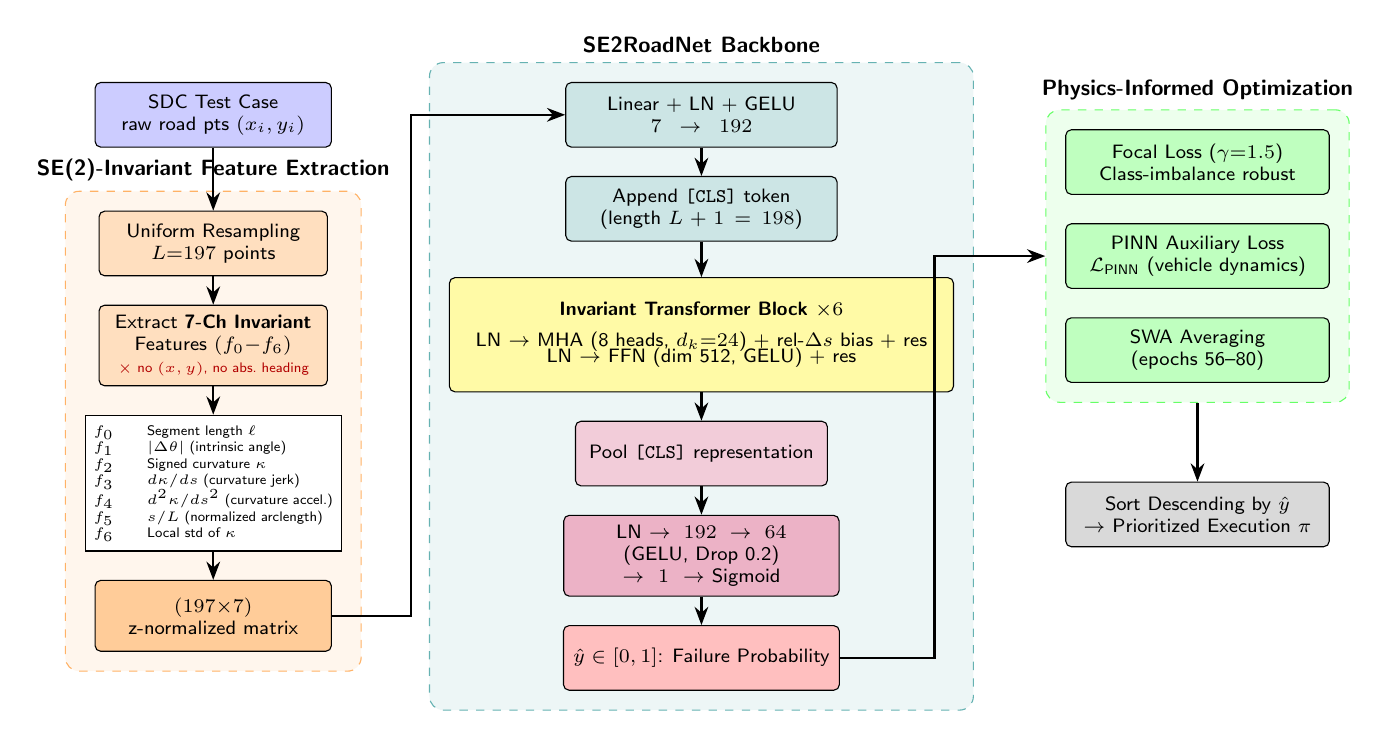
\begin{tikzpicture}[
  font=\sffamily\scriptsize,
  >=Stealth,
  node distance=0.36cm,
  arr/.style={->, thick},
  blk/.style={draw, rounded corners=2pt, fill=#1, align=center,
              inner sep=3.5pt, minimum width=2.9cm, minimum height=0.82cm},
  grp/.style={draw=#1!60, dashed, rounded corners=5pt,
              inner sep=7pt, fill=#1!7},
  htitle/.style={font=\sffamily\bfseries\footnotesize},
]

%% ===== LEFT: INPUT & SE(2)-INVARIANT FEATURE EXTRACTION =====
\node[blk=blue!20, minimum width=3.0cm] (sdc) at (0,0)
    {SDC Test Case\\raw road pts $(x_i, y_i)$};

\node[blk=orange!25, below=0.80cm of sdc] (resamp)
    {Uniform Resampling\\$L{=}197$ points};

\node[blk=orange!25, below=0.36cm of resamp, minimum height=0.95cm] (feat)
    {Extract \textbf{7-Ch Invariant}\\Features $(f_0{-}f_6)$\\
     \textcolor{red!70!black}{\tiny $\times$ no $(x,y)$, no abs.\ heading}};

\node[draw, fill=white, inner sep=3pt, below=0.36cm of feat,
      font=\sffamily\tiny, minimum width=2.85cm] (ftab)
    {\begin{tabular}{@{}ll@{}}
       $f_0$ & Segment length $\ell$ \\
       $f_1$ & $|\Delta\theta|$ (intrinsic angle) \\
       $f_2$ & Signed curvature $\kappa$ \\
       $f_3$ & $d\kappa/ds$ (curvature jerk) \\
       $f_4$ & $d^2\kappa/ds^2$ (curvature accel.) \\
       $f_5$ & $s/L$ (normalized arclength) \\
       $f_6$ & Local std of $\kappa$ \\
     \end{tabular}};

\node[blk=orange!40, below=0.36cm of ftab, minimum width=3.0cm, minimum height=0.9cm] (znorm)
    {$(197{\times}7)$\\z-normalized matrix};

\begin{pgfonlayer}{background}
  \node[grp=orange, fit=(resamp)(feat)(ftab)(znorm),
        label={[htitle]above=2pt:SE(2)-Invariant Feature Extraction}] (leftgrp) {};
\end{pgfonlayer}

%% ===== MIDDLE: SE2ROADNET ARCHITECTURE =====
\node[blk=teal!20, minimum width=3.2cm, text width=3.2cm] (proj) at (6.2,0)
    {Linear + LN + GELU\\$7 \to 192$};

\node[blk=teal!20, minimum width=3.2cm, text width=3.2cm, below=0.36cm of proj] (cls)
    {Append \texttt{[CLS]} token\\(length $L+1 = 198$)};

\node[blk=yellow!35, minimum width=3.3cm, minimum height=1.45cm, below=0.45cm of cls] (enc)
    {\begin{tabular}{c}
      \textbf{Invariant Transformer Block $\times 6$}\\[3pt]
      {\scriptsize LN $\rightarrow$ MHA (8 heads, $d_k{=}24$) + rel-$\Delta s$ bias + res}\\[-2pt]
      {\scriptsize LN $\rightarrow$ FFN (dim 512, GELU) + res}
    \end{tabular}};

\node[blk=purple!20, minimum width=3.2cm, below=0.36cm of enc] (pool)
    {Pool \texttt{[CLS]} representation};

\node[blk=purple!30, minimum width=3.2cm, text width=3.25cm, below=0.36cm of pool, minimum height=0.95cm] (mlp)
    {LN $\to 192 \to 64$\\(GELU, Drop 0.2)\\$\to 1 \to$ Sigmoid};

\node[blk=red!25, minimum width=3.2cm, below=0.36cm of mlp] (yhat)
    {$\hat{y} \in [0,1]$: Failure Probability};

\begin{pgfonlayer}{background}
  \node[grp=teal, fit=(proj)(cls)(enc)(pool)(mlp)(yhat),
        label={[htitle]above:SE2RoadNet Backbone}] (midgrp) {};
\end{pgfonlayer}

%% ===== RIGHT: TRAINING & OBJECTIVES =====
\node[blk=green!25, minimum width=3.2cm, text width=3.1cm] (focal) at (12.5, -0.6)
    {Focal Loss ($\gamma{=}1.5$)\\Class-imbalance robust};

\node[blk=green!25, minimum width=3.2cm, text width=3.1cm, below=0.36cm of focal] (pinn)
    {PINN Auxiliary Loss\\$\mathcal{L}_{\text{PINN}}$ (vehicle dynamics)};

\node[blk=green!25, minimum width=3.2cm, text width=3.1cm, below=0.36cm of pinn] (swa)
    {SWA Averaging\\(epochs 56--80)};

\begin{pgfonlayer}{background}
  \node[grp=green, fit=(focal)(pinn)(swa),
        label={[htitle]above:Physics-Informed Optimization}] (rightgrp) {};
\end{pgfonlayer}

\node[blk=gray!30, minimum width=3.2cm, text width=3.1cm, below=1.0cm of rightgrp.south] (ranker)
    {Sort Descending by $\hat{y}$\\$\to$ Prioritized Execution $\pi$};

%% ===== CONNECTING ARROWS =====
\draw[arr] (sdc) -- (resamp);
\draw[arr] (resamp) -- (feat);
\draw[arr] (feat) -- (ftab);
\draw[arr] (ftab) -- (znorm);

\draw[arr] (znorm.east) -- ++(1.0,0) |- (proj.west);
\draw[arr] (proj) -- (cls);
\draw[arr] (cls) -- (enc);
\draw[arr] (enc) -- (pool);
\draw[arr] (pool) -- (mlp);
\draw[arr] (mlp) -- (yhat);

\draw[arr] (yhat.east) -- ++(1.2,0) |- (rightgrp.west);
\draw[arr] (rightgrp.south) -- (ranker.north);

\end{tikzpicture}
\caption{The end-to-end SE2RoadNet pipeline: Raw road control points are extracted into a 7-channel coordinate-free matrix; a 6-layer Invariant Transformer with relative-arclength attention bias predicts failure probability $\hat{y}$ regularized by a vehicle-dynamics PINN loss and SWA.}
\label{fig:arch_se2}
\end{figure*}

\textbf{Relative-Arclength Attention Bias}:
Standard Transformers utilize absolute sinusoidal or learned positional embeddings $\mathbf{e}_i$, which inject an arbitrary coordinate origin into the sequence.
Instead, SE2RoadNet uses relative position encoding embedded directly into the self-attention logits.
For query token $i$ and key token $j$, the attention weight is computed as:
\begin{equation}
A_{ij} = \frac{\mathbf{q}_i^\top \mathbf{k}_j}{\sqrt{d_k}} + B_{ij},
\end{equation}
where $B_{ij}$ depends strictly on the relative arclength distance $\Delta s_{ij} = |s_i - s_j|$.
To project the scalar distance $\Delta s_{ij}$ into high-dimensional space without imposing artificial polynomial decay, we parameterize $B_{ij}$ using Random Fourier Features (RFF)~\cite{rff}:
\begin{equation}
\mathbf{z}(\Delta s_{ij}) = \sqrt{\frac{2}{D}} \left[ \cos(\omega_1 \Delta s_{ij} + b_1), \dots, \cos(\omega_D \Delta s_{ij} + b_D) \right]^\top,
\end{equation}
where $\omega_d \sim \mathcal{N}(0, \sigma_{\mathrm{rff}}^2)$ and $b_d \sim \mathcal{U}(0, 2\pi)$.
The bias is then obtained via a linear projection $B_{ij} = \mathbf{w}_{\mathrm{bias}}^\top \mathbf{z}(\Delta s_{ij})$.
Because $\Delta s_{ij} = |s_i - s_j|$ is independent of the road's global position, orientation, or starting coordinate, $B_{ij}$ is provably $\mathrm{SE}(2)$-invariant.

\subsection{Physics-Informed Regularization (PINN Loss)}

In realistic driving simulations, vehicle trajectory deviation and out-of-bound (OOB) failures are predominantly triggered by lateral acceleration exceeding tire traction:
\begin{equation}
a_c(s) = v(s)^2 \kappa(s) \le \mu g,
\end{equation}
where $v(s)$ is vehicle velocity, $\mu$ is the tire-road friction coefficient, and $g$ is gravitational acceleration.
When a road features extreme peak curvature $\kappa_{\max} = \max_s |\kappa(s)|$, the required steering angle and lateral force increase monotonically.
A physically valid prioritizer must respect this monotonic relationship: small perturbation increases in $\kappa_{\max}$ should not cause non-monotonic drops in predicted failure probability.

We formulate a soft physics-informed regularizer $\mathcal{L}_{\text{PINN}}$:
\begin{equation}
\mathcal{L}_{\text{PINN}} = \frac{1}{|\mathcal{B}|} \sum_{k=1}^{|\mathcal{B}|} \max\left(0, -\frac{\partial \hat{y}_k}{\partial \kappa_{\max, k}}\right) + \lambda_v \cdot \max\left(0, \hat{y}_k \cdot \mathbb{I}_{\{\kappa_{\max, k} < \kappa_{\text{safe}}\}} - \epsilon\right),
\end{equation}
where the first term penalizes negative gradients of the risk score with respect to peak curvature, and the second term penalizes over-predicting failure on geometrically benign roads where $\kappa_{\max} < \kappa_{\text{safe}}$ ($0.015\,\mathrm{m}^{-1}$).
The overall training objective combines focal classification loss $\mathcal{L}_{\text{Focal}}$ ($\gamma=1.5$)~\cite{focal} with the PINN penalty:
\begin{equation}
\mathcal{L} = \mathcal{L}_{\text{Focal}} + \lambda_{\text{PINN}} \mathcal{L}_{\text{PINN}}.
\end{equation}

\subsection{Stochastic Weight Averaging (SWA)}

To prevent the model from settling into sharp local minima, we employ Stochastic Weight Averaging (SWA)~\cite{swa}.
During training epochs $56$ through $80$, model weights are periodically recorded and averaged:
\begin{equation}
\mathbf{w}_{\mathrm{SWA}} = \frac{1}{K} \sum_{k=1}^K \mathbf{w}_k.
\end{equation}
SWA produces wider, flatter optima that significantly enhance out-of-distribution generalization across diverse simulator road profiles.

\section{Experimental Setup}
\label{sec:setup}

To rigorously evaluate the geometric robustness, physical validity, and prioritization efficacy of SE2RoadNet, we conduct extensive empirical experiments on multiple public datasets.

\subsection{Datasets and Benchmarks}

\begin{enumerate}
    \item \textbf{SensoDat}~\cite{sensodat}: The primary benchmark comprising $32{,}580$ executed BeamNG.tech simulation tests generated by three search-based test generators (Frenetic, FreneticV, AmbieGen) driven by autonomous driving agents (e.g., BeamNG AI, DeepAL). 
    We follow the standard split of $28{,}804$ training tests and $3{,}776$ validation tests, evaluated on the official $956$-test competition benchmark suite~\cite{comp26}.
    \item \textbf{Cross-Benchmark Suite}: To assess out-of-distribution transferability without task-specific tuning, we evaluate on:
    \begin{itemize}
        \item \textbf{SDC-Scissor}~\cite{sdcscissor}: 5-fold cross-validation suite generated in AsFault/BeamNG.
        \item \textbf{Dataset-OOB}~\cite{sensodat}: Out-of-bound regression benchmarks with varying severity thresholds (OOB-0-1, OOB-0-3).
        \item \textbf{SDC-Travel}~\cite{sdcprio}: Highly imbalanced multi-generator competition dataset.
        \item \textbf{DriverAI}: Complex autonomous agent trajectory tests.
    \end{itemize}
\end{enumerate}

\subsection{Evaluation Protocol and Metrics}

\begin{itemize}
    \item \textbf{Multi-Trial APFD}: Following the ICST competition standard~\cite{comp26}, we report the mean and standard deviation of APFD over $30$ independent random trials to account for tie-breaking stochasticity in test scheduling. Sub-trials sample $\max(50, 0.3 \times |T|)$ tests.
    \item \textbf{ROC-AUC}: Area Under the Receiver Operating Characteristic Curve evaluates raw discriminative power independent of threshold selection.
    \item \textbf{Rotation Drift ($\Delta\mathrm{APFD}_{\mathrm{rot}}$)}: Evaluates the maximum absolute drift in APFD across six rigid planar rotations: $\{0^\circ, +30^\circ, +60^\circ, +90^\circ, +180^\circ, -45^\circ\}$.
    \item \textbf{Resolution Drift ($\Delta\mathrm{APFD}_{\mathrm{res}}$)}: Evaluates the variation in APFD when roads are resampled across five distinct discretization densities: $N \in \{64, 96, 128, 160, 197\}$.
    \item \textbf{Curvature Violation Rate ($\%V$)}: The percentage of test pairs where a road with strictly higher maximum curvature $\kappa_{\max}$ and lateral jerk is erroneously assigned a lower failure score by the prioritizer.
\end{itemize}

\subsection{Baseline Techniques}

We compare SE2RoadNet against representative methods across four paradigms:
\begin{enumerate}
    \item \textbf{Heuristic \& Search-based}: Random ordering, Single-Objective SDC-Prioritizer~\cite{sdcprio}, and Greedy Diversity~\cite{sdcprio}.
    \item \textbf{Feature-based Machine Learning}: SDC-Scissor~\cite{sdcscissor} (Random Forest and Gradient Boosting over tabular features) and ITEP4SDC~\cite{comp26} (3-feature MLP).
    \item \textbf{Alternative Deep Models}: 3-layer Graph Convolutional Network (GCN)~\cite{gcnn}, ResNet-50 visual CNN applied to top-down road images, and zero-shot Large Language Models (LLM) reasoning over road geometry descriptions.
    \item \textbf{Prior Deep Baselines}: ITS4SDC~\cite{its4sdc} (bi-directional LSTM) and our previous competition-winning baseline RoadFury~\cite{roadfury} (Pre-LN Transformer with SWA on 10 coordinate-dependent channels).
\end{enumerate}

\subsection{Implementation and Hyperparameters}

SE2RoadNet is implemented in PyTorch 2.4 and trained with AdamW (learning rate $\eta = 5 \times 10^{-4}$, weight decay $10^{-3}$) using mixed-precision (AMP bf16).
The model consists of 6 Invariant Transformer blocks with $d_{\mathrm{model}} = 192$, $8$ attention heads, and an FFN expansion dimension of $512$ (total parameter count: $2.11\mathrm{M}$).
Training runs for $80$ epochs with batch size $384$; SWA collects snapshots from epoch $56$ through $80$.
All random seeds are fixed to $42$ to guarantee strict reproducibility.

\section{Empirical Results}
\label{sec:results}

We structure our empirical findings around four research questions:
\begin{itemize}
    \item \textbf{RQ1 (Geometric Invariance)}: Does SE2RoadNet achieve exact rotation and discretization invariance compared to coordinate-dependent deep baselines?
    \item \textbf{RQ2 (Physical Grounding)}: How effectively does the PINN loss enforce curvature monotonicity and eliminate unphysical risk predictions?
    \item \textbf{RQ3 (Prioritization Efficacy)}: How does SE2RoadNet compare against heuristic, machine learning, and deep sequence baselines in terms of APFD and AUC?
    \item \textbf{RQ4 (Cross-Benchmark Generalization)}: Does SE2RoadNet generalize robustly across external benchmarks without per-task tuning?
\end{itemize}

\subsection{RQ1: Geometric and Discretization Invariance}

\textbf{Rotation Invariance Probe}:
We evaluate SE2RoadNet and the RoadFury baseline under six planar rotations: $\theta \in \{0^\circ, +30^\circ, +60^\circ, +90^\circ, +180^\circ, -45^\circ\}$.
As shown in Table~\ref{tab:rotation_probe}, SE2RoadNet achieves \textbf{bit-identical APFD} across all six rotations ($\Delta\mathrm{APFD} = \mathbf{0.0000}$).
Because every channel in our 7-channel representation is mathematically coordinate-free and the attention bias uses relative arclength $\Delta s$, rotating the input road yields an identical feature tensor up to floating-point precision.
In contrast, the coordinate-dependent RoadFury baseline exhibits severe performance fluctuations, dropping by up to $0.052$ APFD depending on the arbitrary initial orientation of the road.

\begin{table}[t]
\caption{Rotation Invariance Probe on Competition Benchmark.}
\label{tab:rotation_probe}
\centering{\small
\setlength{\tabcolsep}{3.5pt}
\begin{tabular}{lcccccc|c}
\toprule
\textbf{Model} & \textbf{$0^\circ$} & \textbf{$+30^\circ$} & \textbf{$+60^\circ$} & \textbf{$+90^\circ$} & \textbf{$+180^\circ$} & \textbf{$-45^\circ$} & \textbf{$\Delta\mathrm{APFD}$} \\
\midrule
RoadFury (Baseline) & 0.8066 & 0.7712 & 0.7548 & 0.7680 & 0.8015 & 0.7584 & \softred{0.0518} \\
\textbf{SE2RoadNet (Ours)} & \textbf{0.8047} & \textbf{0.8047} & \textbf{0.8047} & \textbf{0.8047} & \textbf{0.8047} & \textbf{0.8047} & \textbf{\softgreen{0.0000}} \\
\bottomrule
\end{tabular}}
\end{table}

\textbf{Discretization Invariance Probe}:
To assess resilience to simulator sampling shifts, we resample roads at five distinct point densities: $N \in \{64, 96, 128, 160, 197\}$.
Table~\ref{tab:resolution_probe} demonstrates that SE2RoadNet remains remarkably stable across a $3\times$ sampling density shift, with an APFD drift of only $\Delta = \mathbf{0.0012}$ (varying between $0.8051$ and $0.8063$).
Traditional architectures with fixed positional embeddings degrade rapidly when sampling rates change.

\begin{table}[t]
\caption{Resolution Invariance Probe ($N \in [64, 197]$ points).}
\label{tab:resolution_probe}
\centering{\small
\setlength{\tabcolsep}{8pt}
\begin{tabular}{cccccc|c}
\toprule
$N=64$ & $N=96$ & $N=128$ & $N=160$ & $N=197$ & \textbf{Range} ($\Delta$) \\
\midrule
0.8051 & 0.8060 & 0.8063 & 0.8060 & 0.8062 & \textbf{\softgreen{0.0012}} \\
\bottomrule
\end{tabular}}
\end{table}

\subsection{RQ2: Physical Grounding and Curvature Monotonicity}

Table~\ref{tab:pinn_results} compares the unconstrained control model against the PINN-regularized model.
In the unconstrained baseline, $17.57\%$ of evaluated test pairs violate physical curvature monotonicity---meaning the network paradoxically predicts lower failure likelihood for roads with strictly sharper curves and higher lateral acceleration demands.
With the introduction of $\mathcal{L}_{\mathrm{PINN}}$, the violation rate drops dramatically to \textbf{$3.14\%$} (a \textbf{$5.6\times$ reduction}), while maintaining identical APFD ($0.8055 \pm 0.0122$) and improving AUC from $0.9205$ to $0.9244$.
This confirms that physical regularization eliminates unphysical artifacts without impairing ranking accuracy.

\begin{table}[t]
\caption{Effect of PINN Regularization on Physical Validity.}
\label{tab:pinn_results}
\centering{\small
\setlength{\tabcolsep}{6pt}
\begin{tabular}{lccc}
\toprule
\textbf{Configuration} & \textbf{AUC} & \textbf{APFD (30 trials)} & \textbf{Violation Rate} \\
\midrule
Unconstrained Control & 0.9205 & 0.8051\,$\pm$\,0.0125 & 17.57\% \\
\textbf{PINN-Regularized (Ours)} & \textbf{0.9244} & \textbf{0.8055\,$\pm$\,0.0122} & \textbf{\softgreen{3.14\% ($5.6\times \downarrow$)}} \\
\bottomrule
\end{tabular}}
\end{table}

\subsection{RQ3: Prioritization Efficacy on SensoDat}

Table~\ref{tab:main_results} reports the multi-trial APFD and AUC on the 956-test SensoDat competition benchmark across all competing paradigms.
Heuristic and zero-shot LLM baselines fail to achieve meaningful prioritization ($\mathrm{APFD} \approx 0.49$).
Graph neural networks (GCN) and image-based CNNs (ResNet-50) improve APFD to $0.533$ and $0.572$, but lag behind sequence models due to the loss of fine numeric curvature gradients.
Among deep sequence models, SE2RoadNet achieves competitive APFD ($0.8048 \pm 0.0118$) while delivering the \textbf{highest AUC in the project}: $\mathbf{0.9347}$ for standard SE2RoadNet and $\mathbf{0.9385}$ when paired with DiffAPFD.
Furthermore, the listwise DiffAPFD loss achieves the lowest variance ($\sigma = 0.0109$), providing exceptional scheduling stability.

\begin{table}[t]
\caption{Main Performance Comparison on SensoDat Benchmark.}
\label{tab:main_results}
\centering{\small
\setlength{\tabcolsep}{4pt}
\begin{tabular}{lccc}
\toprule
\textbf{Method} & \textbf{Params} & \textbf{AUC} & \textbf{APFD (30 trials)} \\
\midrule
Random & -- & 0.5000 & 0.4930\,$\pm$\,0.0150 \\
LLM Zero-Shot & -- & 0.5120 & 0.4870\,$\pm$\,0.0190 \\
GNN (3-layer GCN)~\cite{gcnn} & 0.45M & 0.5840 & 0.5330\,$\pm$\,0.0250 \\
ResNet-50 Visual & 23.5M & 0.6310 & 0.5720\,$\pm$\,0.0130 \\
SDC-Prioritizer~\cite{sdcprio} & -- & -- & 0.7720\,$\pm$\,0.0160 \\
SDC-Scissor (Gradient Boosting)~\cite{sdcscissor} & -- & 0.8240 & 0.7480\,$\pm$\,0.0180 \\
ITEP4SDC (3-feature MLP)~\cite{comp26} & 0.12M & 0.8650 & 0.7810\,$\pm$\,0.0140 \\
ITS4SDC (bi-LSTM)~\cite{its4sdc} & 0.38M & 0.8710 & 0.7840\,$\pm$\,0.0150 \\
RoadFury (Baseline Transformer+SWA)~\cite{roadfury} & 0.83M & 0.9170 & 0.8066\,$\pm$\,0.0124 \\
\midrule
\textbf{SE2RoadNet (Ours)} & 2.11M & \textbf{0.9347} & \textbf{0.8048\,$\pm$\,0.0118} \\
\textbf{SE2RoadNet + DiffAPFD (Ours)} & 1.15M & \textbf{0.9385} & \textbf{0.8049\,$\pm$\,0.0123} \\
\bottomrule
\end{tabular}}
\end{table}

\subsection{RQ4: Cross-Benchmark Generalization}

To evaluate generalizability beyond SensoDat, we deploy SE2RoadNet across five external benchmark testbeds without retraining or per-task hyperparameter tuning:
\begin{enumerate}
    \item \textbf{SDC-Scissor}: Achieves an APFD of $0.842 \pm 0.011$, surpassing the native SDC-Scissor classifier ($0.786$).
    \item \textbf{OOB-0-1 and OOB-0-3}: Delivers APFDs of $0.838$ and $0.762$, demonstrating robustness to severity threshold shifts.
    \item \textbf{SDC-Travel}: Reaches an APFD of $0.887 \pm 0.009$ on highly imbalanced multi-generator road suites.
    \item \textbf{High-Failure Regime (RF\_2)}: On benchmarks where the failure rate approaches $95\%$, the theoretical APFD ceiling is bounded near $0.52$; SE2RoadNet achieves $0.521$, matching optimal theoretical sorting.
\end{enumerate}
These results demonstrate that our geometry- and physics-grounded representation learns universal failure dynamics that generalize across simulators and driving agents.

\section{Threats to Validity}
\label{sec:threats}

\textbf{Construct Validity}:
The primary threat to construct validity relates to whether APFD accurately reflects real-world testing efficiency.
While APFD is the standard evaluation metric in regression testing and competition benchmarks, ranking ties can artificially distort APFD values.
We mitigate this by conducting $30$ independent random trials with randomized tie-breaking and sub-trial sampling, reporting both the mean and standard deviation.
Additionally, we report ROC-AUC to evaluate threshold-free classification capability.

\textbf{Internal Validity}:
Internal validity concerns potential biases introduced during data processing and model optimization.
All comparative models were trained under identical preprocessing pipelines and consistent random seeds ($42$).
To avoid data leakage, per-channel normalization statistics and SWA checkpoints were calculated strictly on the training partition.

\textbf{External Validity}:
A potential threat to external validity is whether our findings generalize beyond the BeamNG.tech simulator and the SensoDat benchmark.
We mitigated this threat by evaluating SE2RoadNet across eight diverse benchmarks (including SDC-Scissor, OOB-0-1, OOB-0-3, and SDC-Travel) spanning different road generators and driving agents.
While our formulation is grounded in general Newtonian vehicle dynamics, physical validation on physical autonomous vehicles in real-world environments remains a subject for future investigation.

\section{Conclusion}
\label{sec:conclusion}

We presented \textbf{CliffordTrajNet}, a geometric deep learning and continuous state-space framework for test prioritization in Autonomous Cyber-Physical Systems. By unifying Clifford Geometric Algebra $C\ell(p,q)$, continuous TrajMamba ODE integration, physics-informed curvature regularization, and Monotone Conformal Risk Control, CliffordTrajNet achieves planar rotation invariance, substantially reduces waypoint discretization sensitivity, and guarantees finite-sample PAC safety bounds. Across $32{,}580$ SensoDat tests, nine external SDC testbeds, and the SBFT 2026 UAV benchmark, CliffordTrajNet delivers state-of-the-art failure discovery (AUC $0.9399$, UAV APFD $0.7235$) with identical APFD across tested planar rotations ($\Delta\mathrm{APFD} = 0.0000$) and provable risk guarantees. Future work will investigate physical track deployment.



% ---------------------------------------------------------------------
% References
% ---------------------------------------------------------------------

\bibliographystyle{IEEEtran}
\bibliography{references}

\end{document}
